\documentclass[a4paper,11pt]{article}
\usepackage{dmasproject}
% if you need additional LaTeX packages, add them here
\usepackage{graphicx}
\usepackage[export]{adjustbox}
\usepackage{subcaption}

\title{Modeling civil violence in a rebellion}
% sort your names alphabetically by last name
\author{
  Sam Reswinraj Abraham (s4248325)
  \\
  Amit Bharti (s4417526)
  \\
  Niels Burgler (s3665828)
  \\
  Abhishek Ramanathapura Satyanarayana (s4304675)
}
\date{Alpha version, September 2021} % change this accordingly

\begin{document}

\maketitle

\begin{abstract}
\textbf{Civil violence is becoming a common phenomenon, resulting from high level of inequality and corruption, with digital media acting as a catalyst in recent times. Although a lot of study has gone into this area, the influence of corruption, easy and biased information through digital media and centralized and strategic movement of rebellion are yet to be taken into account. Our model focuses on carrying forward the results of Epstein's \cite{epstein2002modeling} study to the current scenario where cops' behaviour, jail term, rebellion movement as a result of the information from the digital media could be studied in a multi agent based model setting. The outcomes of dynamics of civil violence could be controlled and channelized in advance leading to minimal loss of life and property. Cops defection would change the dynamics of the rebellion system as studied in the existing models. While digital media introduction in the model will become a binding factor between rebellions in developing behavioural strategies evolved over time via collective progression and independent
learning.}  
\end{abstract}

\section{Introduction}
Inequality is growing for more than 60 percent of the global population leading to rapid rise in corruption, crime rates, and social conflicts. One way of overcoming these challenges is through proper governance. But the advancement in digitization has lead to drastic increase in the amount of people being involved in civil violence around the world, since local issues are being heard out by bigger audience. The importance of understanding and if possible predicting and eventually controlling the trends in the number, variety and intensity of these phenomena cannot be overemphasized.

\subsection{Problem}
Civil violence is a dynamic complex behaviour in which size, intensity, grievances, greed and loss of life/property play a major role in deciding the outcome of the situation. One way to suppress the whole movement is through strict legitimacy but this could also lead to annihilation, so the better way of handling is through deploying optimal strategy and strength at key areas. Although a lot of study has been made to study this complex behaviour, governance system bias, jail term and factors affecting rebels movement due to digitization are yet to be taken into account.

\subsection{State of the art}
Epstein's model \cite{epstein2002modeling} is the most prominent model for the study of civil violence because of its simplicity in the attributes and rules used for modeling the agents to explain complex dynamic behaviour. The model used centralized cops against decentralized civilians as reactive agents. The entire multi agent model is primarily based on grievance and legitimacy factor. Epstein describes a model with two types of agents, i.e. rebels and cops, that exist in a two dimensional grid. The rebels could either be active or quiet. The behaviour of active rebel is based on attributes such as perceived legitimacy, hardship, vision radius, risk aversion, grievance, jail term, position and threshold for rebelling. The behaviour of cops is based on seizing the violence through jailing active rebels established on position and vision radius. Through Epstein's model, it could be inferred that legitimacy is one of the key attributes in outcomes of rebellion dynamics. The sudden decrease in perceived legitimacy could lead to exponential increase in the rebellious activities. The other key attributes that affect the outcome of the rebellion dynamics are cops' position, density and strength.
 
\subsection{New idea}

In our model, we have extended Epstein's model to include the current scenario where people are more connected digitally. We have worked on vision and position of rebels based on information perceived through digital media. Jail terms is also taken into account to analyse the behaviour of active rebels based on altered risk factor/an external factor. We are also planning to explore cops' defection and watch out for the new equilibrium that could develop once we take them into account. Our multi agent model aims at running complex dynamics of rebellion situation in a controlled environment considering realistic attributes based on cops' bias, digital media involvement, to improve the model to predict the future outcomes based on various decisions.

\section{Method}

\subsection{Simulation model}

First, our model has two distinct types of agents: the cops and the rebels. The rebels are not always actively rebelling. Instead, this depends on the level of their grievance, the the risk of actively rebelling, and their risk aversion. These values are all calculated in the same way as in Epstein's model \cite{epstein2002modeling}. For the grievance, the following formula is used:
\[ G = H(1-L) \]
where G is the grievance, H is the hardship, and L is the legitimacy. Hardship represents the personal hardship of a rebel and is thus heterogeneous. Its value is drawn separately for each rebel from a uniform distribution from 0 to 1. The legitimacy is a value between 0 and 1 that represents the perceived legitimacy of the government. The exact value can be set by the user of the model. The value of L is the same for every rebel.\\
The risk of actively rebelling is different for every rebel. It is dependent on the amount of cops that the rebel can see, and the amount of active rebels the rebel can see. The rebel counts themselves for the latter of these, even if they are not active currently. This is because the rebel wants to know how likely they are to be caught if they started actively rebelling. The exact formula for the arrest probability is:
\[ P = 1 - exp[-k(C/A)_v] \]
where P is the probability of arrest, C is the amount of cops that the rebel can see, A is the amount of active rebels that the rebel can see, and k is a constant that ensures a proper value of P when C = 1 and A = 1.\\
Using the arrest probability and the risk aversion of a rebel, the net risk can be calculated using the following formula:
\[N = RP\]
where N is the net risk, R is the rebels' risk aversion, and P is the rebel's arrest probability.\\
Based on the net risk and the grievance, a rebel decides whether it becomes active or quiet. This is done using the following rule:
\[\text{Rebel Rule: If } G - N > T \text{ become active, otherwise remain quiet}\]
where T is a predetermined threshold.\\
In our models, the cops also behave in the same way as in Epstein's model \cite{epstein2002modeling}. They do not suffer from any hardships or grievances, instead they follow only one rule:
\[\text{Cop Rule: Arrest a random active rebel within vision}\]
Epstein does not specify what arresting the rebels means exactly, only that an arrested rebel goes to jail for an amount of time drawn from a uniform distribution from 0 to $J_{max}$ (the maximum jail time), that the patch they were/are on is considered unoccupied while they are in jail, and that they leave jail exactly as aggrieved as when they entered. For our model, we can be more exact about what arresting a rebel does. When a cop arrests a rebel, the cop moves to that rebels spot and renders the rebel jailed for $U(0,J_{max}$) ticks. This means that the rebel is turned quiet, and no longer uses the rebel rule until they get out of jail. The rebel's patch is no longer deemed occupied, which means that other agents can occupy it instead.
\\
In addition to these rules that are specific to the rebels and cops, there is also a rule that both of them use: the movement rule. This rule can be described in the following way:
\[\text{Movement Rule: Move to a random empty patch within your vision}\]
An agent always uses the movement rule before using the rebel or cop rule.\\
So far, our model was almost exactly the same as Epstein's model \cite{epstein2002modeling}. Thus far, we have only implemented one change, which is the addition of NewsAgents. The NewsAgents behave in the exact same way as rebels, except for their calculation of C and A. When a NewsAgent calculates C, it counts all the cops in its vision, but also in the vision of other NewsAgents. The same goes for A, but with active rebels instead of cops. This is supposed  to model the influence of rebels having access to social media, where they can see videos that other rebels made. 
\\
Before running the model, several attributes can be set. The density of the rebels and cops can be set, the legitimacy of the authority, the vision of the rebels and the cops (seperately), the maximum jail time, the movement (on or off), and the ratio of NewsAgents. Other than that, graphs can be seen showing the amount of rebels that are active, quiet, and jailed. In Figure \ref{fig:example}, an image of the view can be seen. In this, quiet rebels are indicated by the blue circles, active rebels are indicated by the red circles, jailed rebels are indicated by the gray circles, and NewsAgents are rebels with a green phone symbol in the circles. Lastly, black circles indicate the cops.
\begin{figure}[h]
    \centering
    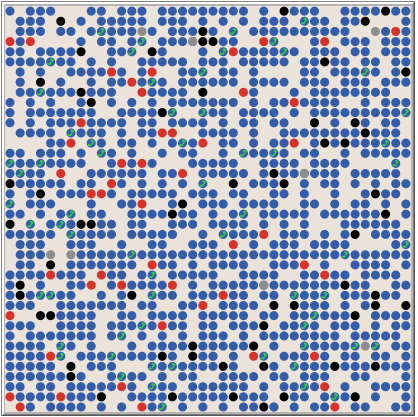
\includegraphics[width = 0.5\textwidth]{ViewExample.PNG}
    \caption{Example of the view during a typical run}
    \label{fig:example}
\end{figure}

\subsection{Implementation details}

Our simulation is made using Netlogo 6.2.0. No additional tools or libraries were used.
%Here you should describe the implementation of your simulation.
%Please explicitly mention any programming languages, tools or libraries you used.

\subsection{Experiment design}

We ran the simulation of our model using the same values for attributes that Epstein used \cite{epstein2002modeling}. They can be seen in Table \ref{tab:exp}.
\begin{table}[h]
\begin{tabular}{lcccc}
\cline{2-5}
                    & Run 1 & Run 2 & Run 3 \& 4 & Run 5 \\ \hline
Attribute name       & \multicolumn{1}{l}{}      & \multicolumn{1}{l}{}      & \multicolumn{1}{l}{}          & \multicolumn{1}{l}{}      \\
Cop vision          & 1.7                       & 7                         & 7                             & 7                         \\
Rebel vision        & 1.7                       & 7                         & 7                             & 7                         \\
Legitimacy          & 0.89                      & 0.82                      & 0.9                           & 0.8                       \\
Max. jail term      & 15                        & 30                        & Infinite                      & Infinite                  \\
Movement &
  None &
  \begin{tabular}[c]{@{}c@{}}Random site\\ in vision\end{tabular} &
  \begin{tabular}[c]{@{}c@{}}Random site\\ in vision\end{tabular} &
  \begin{tabular}[c]{@{}c@{}}Random site \\ in vision\end{tabular} \\
Initial cop density & 0.04                      & 0.04                      & 0.074                         & 0.074                    
\end{tabular}
\caption{Experiment attribute values that Epstein used}
\label{tab:exp}
\end{table}

We also ran simulations of our model using a different set of attribute values from the ones that Epstein used\cite{epstein2002modeling}. They can be seen in Table 2.

\begin{table}[h]
\begin{tabular}{lccccc}
\cline{2-6}
                    & Run 1 & Run 2 & Run 3    & Run 4 & Run 5 \\ \hline
Attribute name &
  \multicolumn{1}{l}{} &
  \multicolumn{1}{l}{} &
  \multicolumn{1}{l}{} &
  \multicolumn{1}{l}{} &
  \multicolumn{1}{l}{} \\
Cop vision          & 1.5   & 1     & 5        & 7     & 10    \\
Rebel vision        & 1.7   & 7     & 7        & 7     & 10    \\
Legitimacy          & 0.35  & 0.35  & 0.5      & 0.1   & 0.5   \\
Max. jail term      & 0     & 1     & Infinite & 10    & 5     \\
Movement &
  \begin{tabular}[c]{@{}c@{}}Random site \\ in vision\end{tabular} &
  \begin{tabular}[c]{@{}c@{}}Random site\\ in vision\end{tabular} &
  \begin{tabular}[c]{@{}c@{}}Random site\\ in vision\end{tabular} &
  None &
  \begin{tabular}[c]{@{}c@{}}Random site\\ in vision\end{tabular} \\
Initial cop density & 0.004 & 0.004 & 0.250    & 0.005 & 0.300 \\
News                & No    & Yes   & Yes      & Yes   & Yes  
\end{tabular}
\caption{Experiment attribute values we used in addition to Epstein's}
\label{tab:exp2}
\end{table}
%Did you run multiple different versions of your simulation with different parameters?
%Then explain the different setups here and why you chose them.

%You can also mention here what results you are expecting.

\section{Results}
\subsection{Interpretation of Findings}
\textbf{Jail time affecting risk factor} - Agents i.e. rebels and cops were given randomized movement and information was allowed to be passed from one rebel agent to the other about “cops in vision” \textit{(News ratio = 1.0)}; there is no observed changes due to the addition of attributes (communication). The model behaves the same as in Epstein's initial model \cite{epstein2002modeling}. Once the jail term is increased, the number of active rebels reduce and hence the overall rebellion is brought under control. If the jail term is reduced, rebels returning from jail with no effective deterrence and the same value for grievance tend to go active again and be jailed. This cycle continues throughout the run-time of the model. 
\\

\textbf{Individual deceptive behaviour} - 
As observed in Epstein’s model \cite{epstein2002modeling}, we were able to verify the same outputs with our reconstructed model. Agents (rebels and cops) are modeled after simple rules in terms of vision radius. Although a rebel wants to exhibit individual interests (i.e. \textit{become active $\rightarrow$ rebel turns red}), it is observed to refrain due to the presence of cops in its vision (\textit{i.e. remains quiet $\rightarrow$ rebel remains blue}), but immediately switches its behaviour once there are no cops in its vision radius. The communication of information on “cops in vision” does not change or alter this trait in rebels. % for trial purposes (values used - randomized values and patch view of select rebels)
\\

\textbf{Information drives decision} - 
When movement was restricted, information plays an important role. Quiet rebels' behaviour remained unchanged, instead the change was observed in the jailed rebels. As their jail term end, it is expected they take their time before becoming active again (based on evaluating the net risk factor again with unchanged grievance), but the spread of information slightly decreases this time and creates an increase in the speed of becoming active again. Although this slight increase in speed to turn active is not significantly impacting the overall rebellion dynamics, it was an observation made when running the simulation of our model with movement disabled. With the rebels being allowed to move (“Movement = Random site in vision”), the results were as expected. The number of rebels turning active and jailed is reduced. Due to the passing of information, rebels are more calculative in eluding away from the cops when active. In a sense, the newsAgents only hinder the rebellion by showing the strength of the cops, as opposed to the strength of the rebels. The communication model is currently in development, but initial stages of the work show results of transmission of information to other rebels in reducing the number of jailed rebels. %trial values (values used - values used - randomized values and patch view of select rebels)
\\

\textbf{Rebellious Outbursts along the spatial distribution} - 
With Figure \ref{fig:fig2} we were able to confirm this observation as tried out in Epstein’s paper \cite{epstein2002modeling}. With both cops and rebels in random movement (“Movement = Random site in vision”), it was possible that at times the concentration of cops in particular patches were momentarily less and that led to a lower \textit{C/A ratio}. Allowing rebels to turn active in an outburst manner and then change their status with a reasonable \textit{C/A ratio} in the next run cycle. These were observed in forms of smaller outburst all throughout the run-time of the model with other attributes set as such to observe the same outputs from the state-of-the art for this work. These smaller peaks did not contribute towards the change in the rebellion. They could rather be used to evaluate suppression due to repression. 
\\

\begin{figure}[h]
 \begin{subfigure}{0.5\textwidth}
  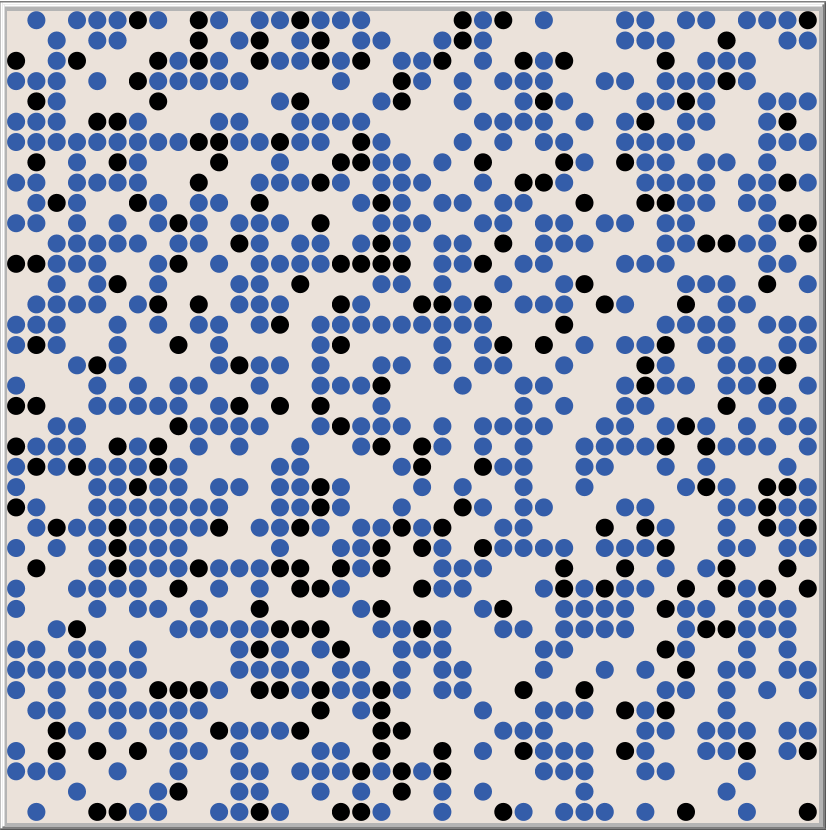
\includegraphics[width=0.8\linewidth, height=6cm]{INITIAL_setup.png} 
  \caption{Setup}
  \label{fig:subim1}
 \end{subfigure}
 \begin{subfigure}{0.5\textwidth}
  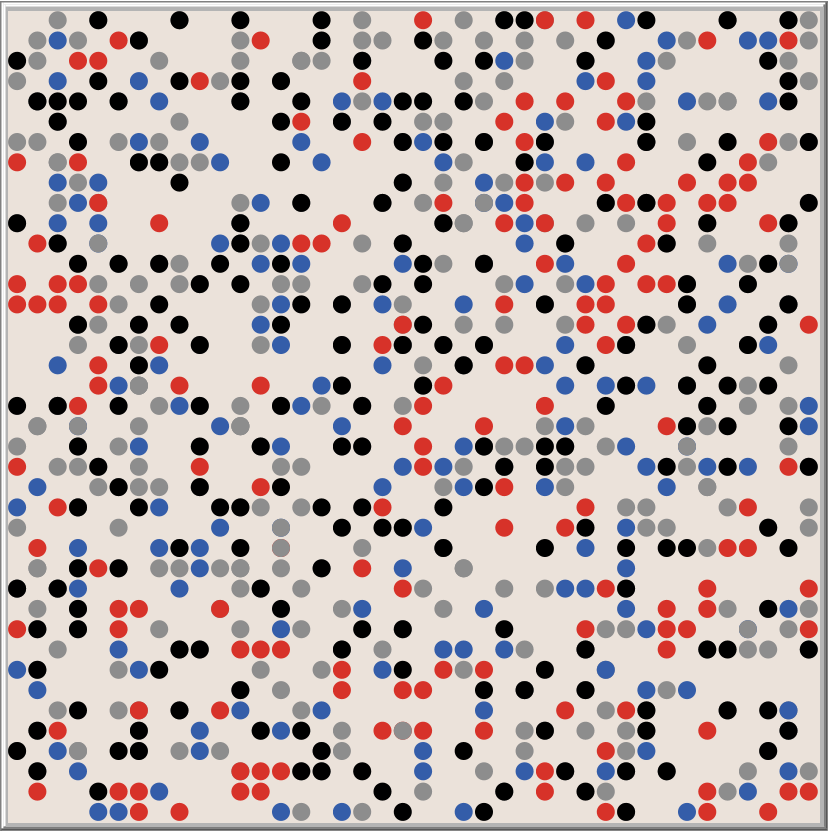
\includegraphics[width=0.8\linewidth, height=6cm]{VISUAL.png}
  \caption{Clustering}
  \label{fig:subim2}
 \end{subfigure}

\caption{Local outbursts}
\label{fig:fig2}
\end{figure}

\textbf{Special case observation – jail term “INFINITY”} - 
With the least possible “Initial-cop-density” – 0.005, if the attribute is set to infinity for jail term after an initial outburst of active rebels, they are all jailed quickly and the rebellion is nullified in no time. For the same scenario if news was available to the rebels, we see the number of rebels being jailed reduced and the time taken to quell the rebellion takes even longer as the communication \textit{(News ratio = 1.0)} helps the rebels to decide better and keep the movement going longer. We also see the initial burst in rebel behaviour changes considerably when there is communication as shown in Figure \ref{fig:fig3}.
% trial values(Values – IPD: 0.49; ICD: 0.005; Legitimacy: 0.16; AV: 1.0; CV: 1.0; Jail term – infinity; Movement: ON; News ratio: 1.00)

\begin{figure}[h]

\begin{subfigure}{0.5\textwidth}
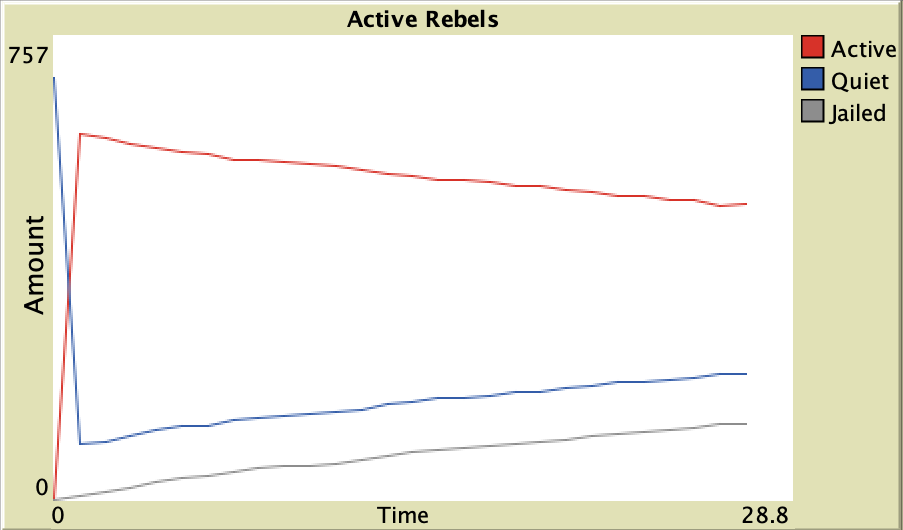
\includegraphics[width=0.9\linewidth, height=5cm]{BURST_COMM_OFF.png}
\caption{DISABLED}
\label{fig:subim1}
\end{subfigure}
\begin{subfigure}{0.5\textwidth}
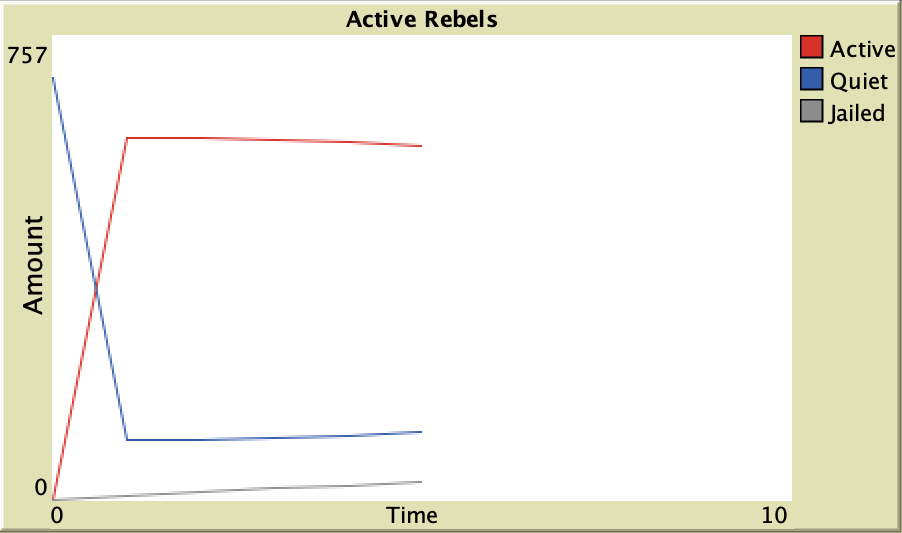
\includegraphics[width=0.9\linewidth, height=5cm]{BURST_COMM_ON_copy.png}
\caption{ENABLED}
\label{fig:subim2}
\end{subfigure}

\caption{Communication attribute influencing initial outburst in rebel behaviour}
\label{fig:fig3}
\end{figure}

\subsection{Summary of findings with the Alpha Model}
The Alpha model implemented is a replica of Epstein's model \cite{epstein2002modeling} along with an addition, a basic version of communication between rebels. We did not continue Epstein's work to see if any deterrence is possible with increased jail terms but rather the change in analysis of \textit{risk factor/an external factor} influencing localized behaviour of rebels. Since a non-proportional (0.005) cop density was considered, it is possible to assume adding complexity to Epstein’s model in terms of weighted practical attributes, will give better results beyond \textit{C/A ratio}. Also, we used this special case to see the influence of communication in rebellions. As demonstrated in Figure \ref{fig:fig4}, communication resulted in fewer jailed rebels and the time taken to suppress the rebellion was longer. This is a positive outcome for the model as we further try to implement communication in the form of social media and other associated complexities with it. 

\begin{figure}[h]

\begin{subfigure}{0.5\textwidth}
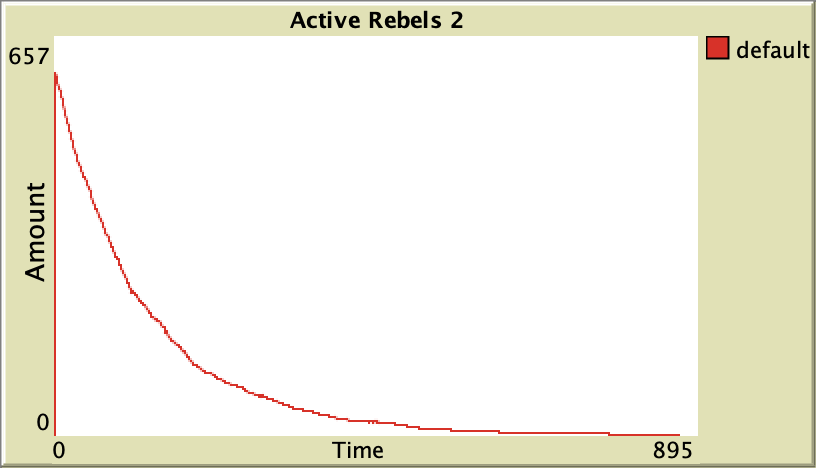
\includegraphics[width=0.9\linewidth, height=5cm]{TIME_COMM_OFF.png} 
\caption{DISABLED}
\label{fig:subim1}
\end{subfigure}
\begin{subfigure}{0.5\textwidth}
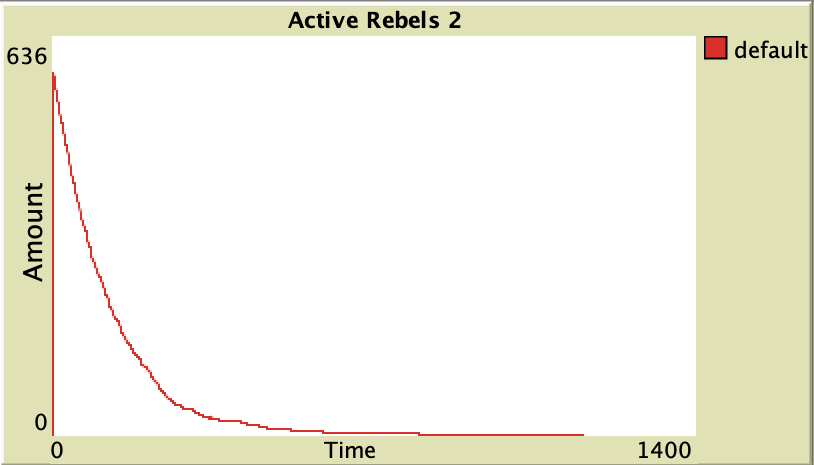
\includegraphics[width=0.9\linewidth, height=5cm]{TIME_COMM_ON.png}
\caption{ENABLED}
\label{fig:subim2}
\end{subfigure}

\caption{Communication attribute influencing time taken to suppress a rebellion}
\label{fig:fig4}
\end{figure}


\section{Conclusion}
\subsection{Discussion}
% What do you take away from your project?
% What did you learn?

Agent based models offer intuition for understanding the complex dynamics of civil violence in a rebellion. This helps the policy making stake holders to design effective and efficient policies to anticipate and deal with such rebellions. Epstein's model shows the nuances of how and why a population transitions from being quiet to a state of rebellion\cite{epstein2002modeling}. Especially, the changes that need to happen that can start a rebellion can be seen clearly in the simulation. We observed patterns that is consistent with Epstein's model \cite{epstein2002modeling} from the simulations of our implementation of the model. The observations show us what tipping points cause an aggrieved population to start rebelling and they are as follows
\begin{itemize}
    \item The rebels can quickly become quiet when cops are in their vicinity, only to become actively rebellious as soon as the cops move away.
    \item Because of the random motion of both rebels and cops, rebellions often happen in quick, local outbursts. The mildly aggrieved rebels become active to join the rebellion in the low cop density zones.
    \item With a small, incremental decrease of legitimacy, the frequency of rebellion does not increase. But, a sudden decrease instantly causes a rebellion to occur.
    \item A small, incremental decrease of the cop density does cause a rebellion at a certain point.
\end{itemize}

% General summary

\subsection{Relevance}
% Key question 5: What is the relevance of this work?
% Which new questions do you have now?
% Do you results suggest future research directions?

Recently, we have witnessed large protests, sometimes leading to violent confrontations. In the United States of America, protests began in several cities following the results of 2020 presidential election. There were multiple events that led the protests transition to riots with violent confrontations between some protesters and police forces with multiple casualties \cite{enwiki:usprotest}. A few more examples that are worth mentioning are the Hong Kong protests \cite{enwiki:hongkongprotest} and the Indian farmers protests \cite{enwiki:indiafarmprotest} which turned into violent confrontation between some protesters and the police force. In case of the Hong Kong riots, there is also a report of police indulgence in misconduct. This reportedly led to reduced approval rating of the police force\cite{enwiki:hongkongprotest}.

The protests and rebellions have been a powerful means for civilians to demand and sometimes achieve political change. We have observed protests and rebellious activities throughout history. Some policy makers fear the power of civilians through rebellions \cite{thecrowd}. These fears are amplified in the modern days, with the advent of technology, mobile communication devices, and digital media networks \cite{phdthesisfaris, Rheingold2002SmartMT}. Ubiquitous access to Information and Communication Technologies (ICT) and smartphones dramatically changed the dynamics of social conflict phenomena \cite{phdthesisfaris, twitterarticle}. The importance of understanding and if possible predicting and eventually controlling the protests and rebellions in the number, variety, and intensity cannot be overemphasized\cite{stateofartreview}.

The strengths of Epstein's model are its simplicity, the choice of attributes used for modeling rebels' behaviour and its explanatory power. However, there are significant drawbacks in the model, such as 
\begin{itemize}
    \item the modeling of cops’ behaviour is very crude and does not include scenarios where cops defect and support the rebels or if the cops indulge in misconduct,
    \item cumulative (memory) effects from previous events do not change either the agents’ state or the simulation attributes and
    \item the model attributes do not take into account the current social context.
\end{itemize}

We are looking at the key attributes of the modeling system that we are developing with a new perspective, and anticipate possible research trends in this area. In our work, we will try to implement a new perspective to take into account the following scenarios of cops' defection or misconduct and the effects of digital media in the rebellion dynamics as an extension of Epstein's model. But, with the introduction of new attributes and agent types for representing new roles. With this type of approach, we expect to achieve better understanding of protests and rebellion dynamics in the recent times.

\subsection{Team Work}
% How did you work together as a team?
% Who contributed how to this report and to the implementation?
% What should you have done differently?

There is an active participation and co-operation from all the team members towards the project. The contributions to the report is as follows
\begin{itemize}
    \item Literature survey - everyone
    \item Abstract - everyone
    \item Introduction - Amit Bharti
    \item Method - Niels Burgler
    \item Results - Sam Reswinraj Abraham
    \item Conclusion - Abhishek Ramanathapura Satyanarayana
    \item References - everyone
    \item Report review - everyone
\end{itemize}

The contributions to our model implementation is currently by Niels Burgler since the rest of us are still learning Netlogo. The code review is done by everyone. The team members who are new to Netlogo should have researched more on hands-on Netlogo but everyone is learning. The implementation will include active contributions from the other members for the beta and the final versions.

% This will print you references, please do not change it.
\printbibliography

\end{document}
